\chapter{Implementation}
The objective of this part of the project was to implement an immersive replication of \acp{ASC} induced by classical psychedelics. In order to achieve a high degree of immersion, our solution was designed to be intended for immersive \ac{VR} systems with \acp{HMD}. Our solution will be referred to with \textit{``the application''} or \textit{``our application''} for the rest of this document.

To represent the \acp{ASC} of classical psychedelics objectively, we had to resort to modelling only the ``perceptual level'' stage of the psychedelic experience (as seen in figure \ref{fig:temporal-dynamics}), as further stages require subjective personalization of content, and aspects less suitable for replication via immersive \ac{VR}, such as cognitive effects and the suppression of the \textit{phenomenological ego}.

\section{Design of the Application}
The application was designed primarily for the evaluation of the implemented replication. The development of the application consisted of 3 distinct parts:

\begin{enumerate}
    \item \textbf{The environment}: A virtual scene that should look as realistic as possible.
    \item \textbf{The replication}: Implementation of the effects themselves.
    \item \textbf{Adaptation for testing}: Getting the application ready for a study, that might measure the impact of the replication on the human mind.
\end{enumerate}

\subsection{Safety}
In order to ensure our application's users safety, we have consulted the \textit{Recommendations for good scientific practice and the consumers of VR-technology} \autocite{madary2016real}. The application was developed according to these recommendations.

Mainly, we don't expect the developed application to have lasting traumatic effects on the users; instead, we believe that this medium may be a suitable way to explore aspects of psychedelic-induced \acp{ASC} while minimizing those risks.

Further, we've taken safety and intuitiveness into account while designing the controls and choosing a suitable testing area for experimentation with \ac{VR} (the ``\ac{VR} play space'').

Finally, the application must be automated, so that the administrator may assist the user and ensure their safety during the usage of the application.

\subsection{Interaction}
Interaction with the scene via hand-held controllers was removed entirely, as we felt that the currently available consumer \ac{VR} technology does not implement a realistic, consistent, universal and intuitive solution for interaction with the virtual scene. For example, in \ac{VR} applications, interactions are usually implemented so that if a user takes a hand-held controller to a dynamic physics-enabled object, they may be able to pick it up by pressing or holding a trigger on the hand-held object, which makes the object stick or snap to the virtual representation of the controller in the scene. While this solution may be suitable for \ac{VR} games, it is still understood as a simplification.

As an alternative, one may consider using force feedback haptic gloves, and given a sufficient physically based simulation, it may be possible to implement realistic interactions with virtual objects. However, even such gloves apply force feedback only to the fingers and not the entire body, making it impossible to, for example, lean against virtual objects.

In any case, no such force feedback haptic gloves were available to us for this project, and so interaction was entirely foregone, in the interest of keeping the simulation focused mainly on the replication, rather than an unrealistic implementation of interactions.

\subsection{Virtual Scene Creation}
Given the goal of creating as realistic of a scene as possible, as well as no financial budget for this project, we ended up choosing \fref{https://web.archive.org/web/20220514231756/https://www.unrealengine.com/en-US}{\acf{UE4}} as the game development engine to develop our \ac{VR} application with. \ac{UE4} is free to use for projects with a lifetime gross revenue below \$1 million USD, and we have no plans to monetize it. Additionally, the choice of \ac{UE4} makes it possible to use the \fref{https://web.archive.org/web/20220514233901/https://quixel.com/megascans}{Quixel Megascans} 3D asset library for free within \ac{UE4}, due to special licensing as a result of the acquisition of Quixel by \fref{https://web.archive.org/web/20220514235540/https://www.epicgames.com/site/en-US/home}{Epic Games}, the developer of \ac{UE4}.

The virtual scene was created with the intended \textit{\ac{VR} play space} in mind, which was measured to be about $3.5\times3.5 \:\si{m^2}$ large. The virtual scene contains visual cues of the \textit{play area} borders in the form of 3D assets; specifically, the \textit{play area} is surrounded by a railing and tall rock, communicating to the user, that these objects should not be passed through.

The choice was made to create an outdoor scene, as the surrounding nature might provide a more pleasant environment than an indoor scene. However, our implementation is in no way limited to outdoor scenes only.

At first, we attempted to create a forest scene, but quickly ran into performance issues while trying to render a densely populated forest on a \ac{HMD}, which requires at least 2 views rendered at typically higher resolutions than a regular desktop screen, ideally with at least 90 \acs{FPS} (the native refresh rate of the \ac{HMD}). Delivering a consistent framerate is a requirement, as low framerates and stuttering may cause motion sickness.

It was then decided to abandon the idea of a forest scene and, instead, use a \ac{HDRI} panoramic photograph as a background (hereinafter ``panoramic background'') for the scene. It is important to note, that a panoramic background has no depth information. This drawback can be mitigated by making only the very distant parts of the panoramic background visible to the user, so that the illusion of the panoramic background being realistic is not broken. The illusion relies on the fact that binocular disparity is low for distant objects.

Close parts of the panoramic background can be hidden with 3D assets suitable for the environment. To minimize the area that needed to be hidden, we have chosen a mountainside panoramic background (see figure \ref{fig:cannon}).

\begin{figure}[H]
    \centering
    \ifgraphics
        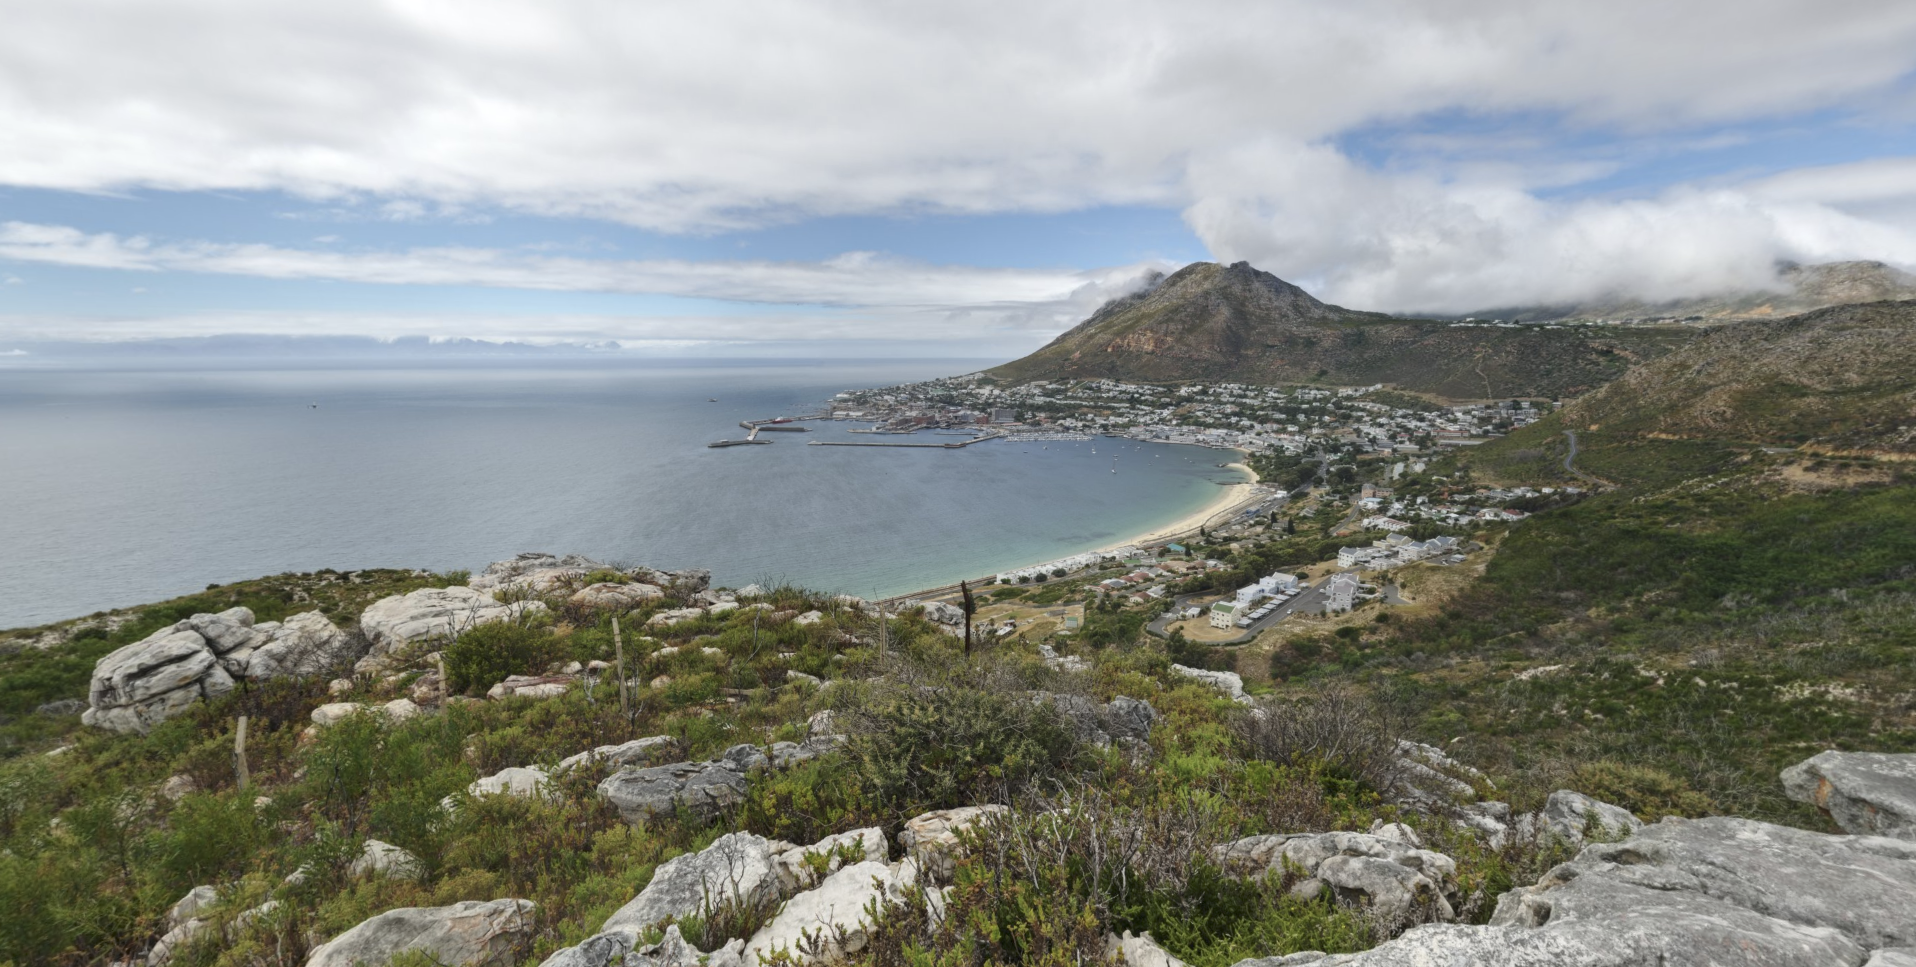
\includegraphics[width=0.95\textwidth]{img/cannon.png}
    \fi
    \caption{The chosen panoramic background ``Cannon''\cczerofootnote{Greg Zaal} available on \fref{https://web.archive.org/web/20220515010919/https://polyhaven.com/a/cannon}{Poly Haven}.}\label{fig:cannon}
\end{figure}

The final scene contains a flat patch of grass and other low foliage the size of the \textit{play area}, containing a wooden bench with some gardening tools. The grass patch is surrounded with rock formations and a rocky stairway leading towards it. Beyond the railing, there is a nice view of the sea cove.

\begin{figure}[H]
    \centering
    \ifgraphics
        TODO: image of the scene
        % 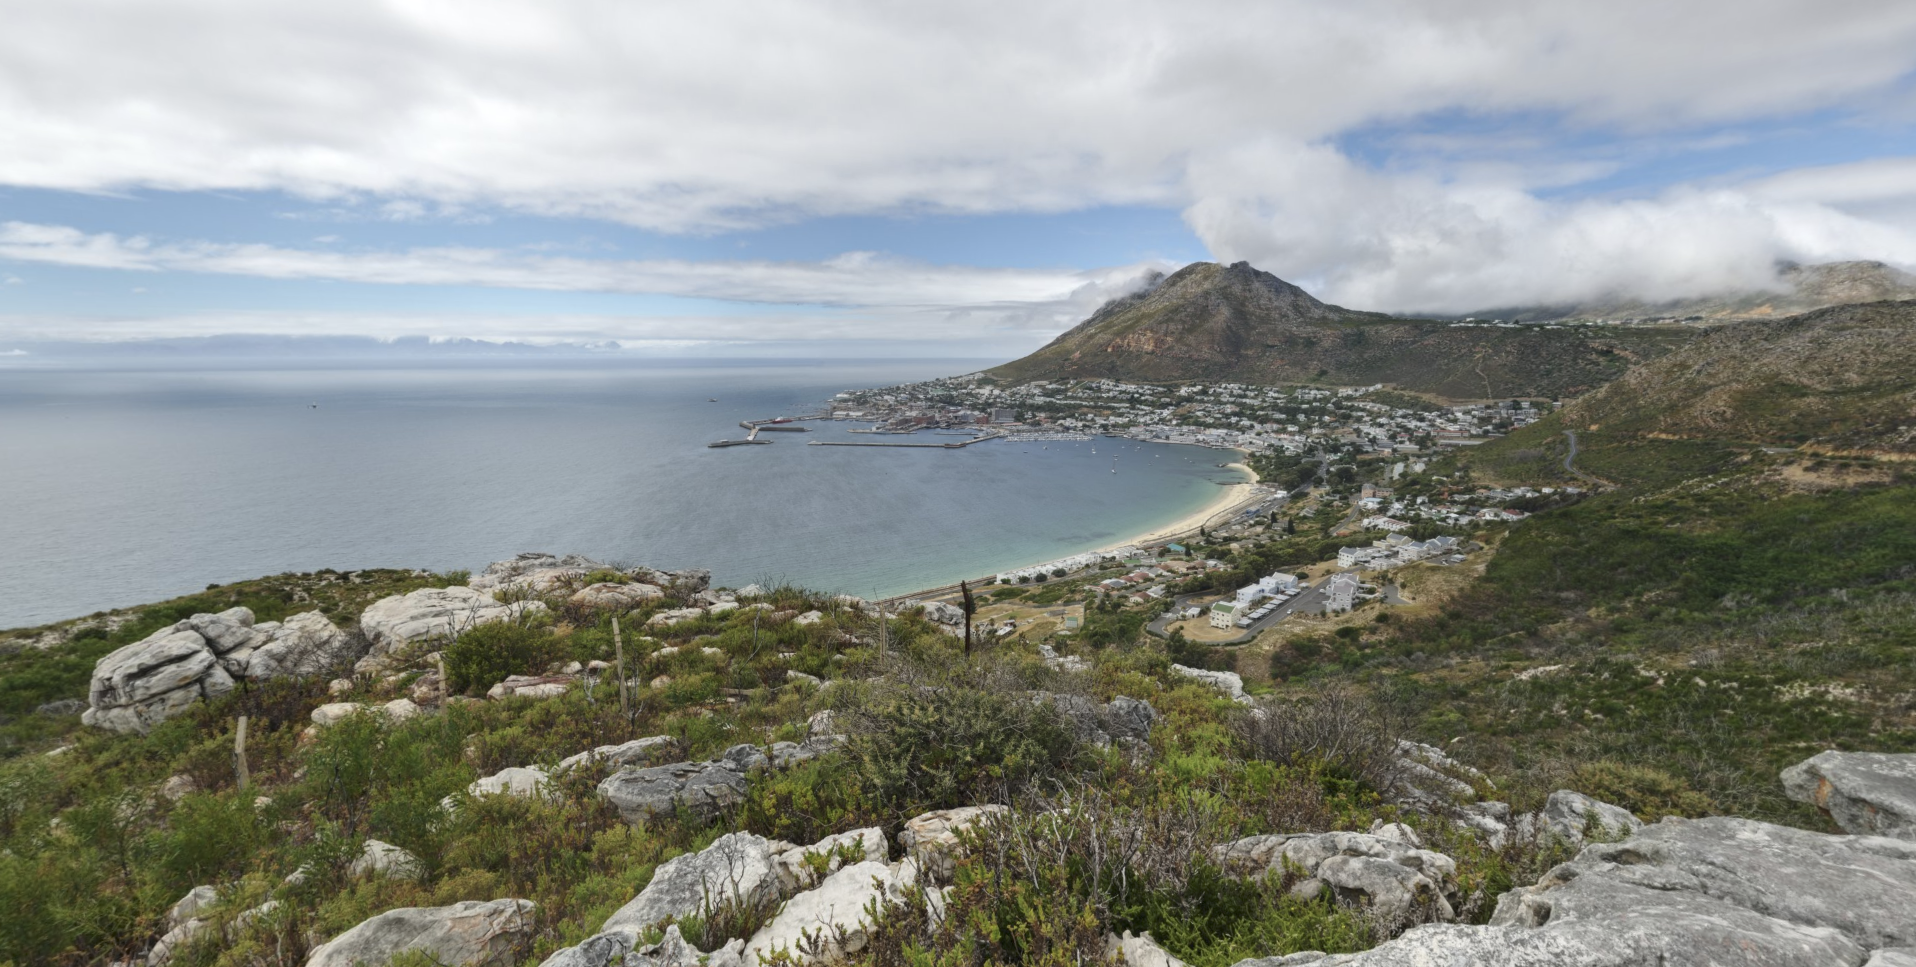
\includegraphics[width=0.95\textwidth]{img/cannon.png}
    \fi
    \caption{A preview of the resulting scene.}\label{fig:scene-preview}
\end{figure}

\section{Implementation of Replications}
The following replications are modelled after surveys of the phenomenology of psychedelic states \autocites{preller2016phenomenology}{kometer2016serotonergic} and personal reports \autocite{kleinman1977comparison}.

\subsection{Spatial Effects}
The spacial effects of this section are a form of a vertex shader, or part thereof. \ac{UE4} has a concept of so-called ``materials'' -- assets that can be applied to meshes to control the visual look of 3D assets. \ac{UE4} materials are defined using a built-in visual programming node graph. While this approach of specifying \ac{GPU} shader logic allows for tighter integration with \ac{UE4}'s rendering engine and its lighting model, it makes it difficult to use conventional shading languages such as \ac{GLSL} or \ac{HLSL}. The usage of conventional shading languages is sometimes desirable, because the provided material node graph editor cannot, by design, express some control flow constructs, such as loops.

However unwieldy, it is possible to use \ac{HLSL} code in material graphs, in \ac{UE4}. The directory of our custom \ac{HLSL} shader files must be properly registered in the engine via an engine plugin \autocite{synthenz2021shaderdir}. The shader files can then be referenced from within ``custom'' nodes of the material node graph editor.

\subsubsection{Depth Perception Distortion}
This replication simulates the distorted perception of depth, micropsia, and macropsia \autocites{fischer1970psilocybin}{dittrich1998standardized}{hill1969effects}{hill1973induction}.

Our replication of the depth perception distortion is implemented as a world-space vertex shader. Even though certain distortions in screen-space may also result in the distortion of depth perception, we chose our approach to achieve better control over the shape of the rendered geometry.

\subsubsubsection{First Attempt}
Our first attempt made use of a self-similar, bijective and continuous function $f$ to modify the distance of vertices from the \ac{HMD}. The self-similarity is required to ensure that no self-intersection of geometry occurs, after the offset has been applied.

\begin{equation}
    \scalebox{1.5}{
        $f(r) = a^{\frac{1}{\pi}\sin(\pi \log_a{r}) + \log_a{r}}$
    }
    \label{eq:depth-perception-f}
\end{equation}

Where $a \in (1; +\infty)$.

The interesting property of self-similarity results in the maximum offset being directly proportional to the distance of the \ac{HMD}. The graph of the function can be seen in figure \ref{fig:depth-perception-f}.

\begin{figure}[H]
    \centering
    \ifgraphics
        {
            \def\consta{1.5}

            \subfloat[\centering Modified distance from the \ac{HMD}. Green line corresponds to the identity function for reference.]{
                \begin{tikzpicture}
                    \begin{axis}[
                        xlabel style={align=center},
                        ylabel style={align=center},
                        xlabel=$r$\\Original Distance from \ac{HMD},
                        ylabel=Modified Distance from \ac{HMD}\\$f(r)$,
                        samples=1000,
                        grid,
                        thick,
                        domain=0:5,
                        xmin=0,
                        xmax=5,
                        ymin=0,
                        ymax=5,
                        legend pos=outer north east,
                        no marks,
                        unit vector ratio={1, 1},
                    ]
                    \addplot+[black!30!green, fill opacity=0.7] gnuplot {x};
                    \addplot+[black] gnuplot {sgn(x) * (\consta)**((1/pi) * sin(pi * log(abs(x)) / log(\consta)) + log(abs(x)) / log(\consta))};
                    \end{axis}
                \end{tikzpicture}
            }

            \subfloat[\centering Distance offset from the \ac{HMD}. Green line corresponds to the X axis for reference. Note that the maximum distance offset is directly proportional to the distance from the \ac{HMD}.]{
                \begin{tikzpicture}
                    \begin{axis}[
                        xlabel style={align=center},
                        ylabel style={align=center},
                        xlabel=$r$\\Original Distance from \ac{HMD},
                        ylabel=Distance Offset from \ac{HMD}\\$f(r) - r$,
                        samples=1000,
                        grid,
                        thick,
                        domain=0:5,
                        xmin=0,
                        xmax=5,
                        ymin=-1,
                        ymax=1,
                        legend pos=outer north east,
                        no marks,
                        unit vector ratio={1, 1},
                        ytick = {-1, 0, 1},
                    ]
                    \addplot+[black!30!green, fill opacity=0.7] gnuplot {0};
                    \addplot+[black] gnuplot {(sgn(x) * (\consta)**((1/pi) * sin(pi * log(abs(x)) / log(\consta)) + log(abs(x)) / log(\consta))) - x};
                    \end{axis}
                \end{tikzpicture}
            }
        }
    \fi
    \caption{First attempt at distorting depth perception, unused in the final application. The function $f$ from equation \ref{eq:depth-perception-f} modifies the distance of vertices from the \ac{HMD}. Parameter $a = 1.5$.}\label{fig:depth-perception-f}
\end{figure}

Although this first iteration resulted in visually enticing results, we also noticed that it caused motion sickness in \ac{VR}, particularly during the user's movement. We believe the motion sickness was caused by clusters of geometry moving with the position of the \ac{HMD}, as if attracted to it, and caused a discrepancy between the user's vestibular system and the visual information.

Another disadvantage of this solution is its predictability and the synthetic look caused by its uniformity.

\subsubsubsection{Final Solution}\label{sec:noise}
In order to break up clusters of similarly affected geometry, we decided to use procedural noise. Procedural noise has been used for the generation of textures \autocite{perlin1985image}, and would be suitable to create a less predictable, more chaotic effect.

There are various kinds of procedural noise used in computer graphics. We found Simplex noise \autocite{olano2002simplex} to be suitable for our use-case, particularly for its $\mathcal{O}(n^2)$ time complexity in $n$ dimensions, lack of directional artifacts (visual isotropy), and a well-defined continuous gradient.

Let's denote the simplex noise sampling function as $s \colon \mathbb{R}^n \to \mathbb{R}$.

Now that we have a way to sample the noise, we could try to use the noise sample (possibly scaled by a constant) as the offset of the distance of each vertex to the \ac{HMD}, as shown in the previous section. To retrieve the sample, we can use:

\begin{equation}\label{eq:simplex}
    s' \coloneqq s\mleft(\begin{bmatrix}f_sx\\f_sy\\f_sz\\f_tt\end{bmatrix}\mright)
\end{equation}

where $s'$ is the resulting sample, $x$, $y$ and $z$ are spacial coordinates of any point in space (typically the position of a vertex), $t$ is the current time in seconds, and $f_s$ and $f_t$ are space-wise and time-wise frequencies of the noise, respectively.

With the addition of the time coordinate, resulting in 4-dimensional noise, the sampled offset value will change over time. This helps break up the uniformity and predictability of the previous solution.

Unfortunately, we have lost one important property of the previous solution: The fact that the maximum offset was directly proportional to the distance from the \ac{HMD}. We could try to reintroduce proportionality naively by multiplying the sample by the distance $r$:

\begin{equation}
    s' \coloneqq r \cdot s\mleft(\begin{bmatrix}f_sx\\f_sy\\f_sz\\f_tt\end{bmatrix}\mright)
\end{equation}

By this modification, we have effectively changed the amplitude of the noise, yet the frequency remains the same -- and uniform. If we were to use this sample $s'$ as the distance offset, we would cause distant geometry to self-intersect. Therefore, a different solution is needed.

For this task, we may use \ac{fBm}. Before we go into how \ac{fBm} can help resolve this issue, let's briefly describe how it is used in the synthesis of self-similar noise. \Ac{fBm} is a technique of combining layers of noise, while varying their amplitudes and frequencies.

\begin{equation}\label{eq:fbm1}
    s' \coloneqq \frac{1}{k} \sum_{i=0}^{k-1} g^i \cdot s\mleft(l^{i} \begin{bmatrix}f_sx\\f_sy\\f_sz\\f_tt\end{bmatrix} + i \vec{o}\mright)
\end{equation}

In equation \ref{eq:fbm1}, we combine $k \in \mathbb{N}$ layers of simplex noise. The parameter $g \in \mathbb{R}$ (gain) changes the amplitude of each layer, and the parameter $l \in \mathbb{R}$ (lacunarity) changes the frequency of each layer. Typically, $l = \frac{1}{g}$; in that case, we are generating so-called ``pink noise''. The parameter $\vec{o} \in \mathbb{R}^n$ is a coordinate offset applied to each layer, to break up symmetry (a different seed for each layer could also be used).

Now, back to our original problem of keeping the amplitude proportional to the distance from the \ac{HMD}. Instead of using $k$ layers of noise with indices $i = 0, 1, \dots, k - 1$, we can offset the indices by an integer value depending on the distance from the \ac{HMD}. If we do so carefully, we will recover the direct proportionality. We define a real-valued offset $m \colon \mathbb{R} \to \mathbb{R}$:

\begin{equation}
    m(r) = \log_a r
\end{equation}

Where $a \in \mathbb{R}$ is a parameter; more on this later. Then, we can define the rounded-down integer part $j \colon \mathbb{R} \to \mathbb{Z}$ to offset the layer indices with:

\begin{equation}
    j(r) = \lfloor m(r) \rfloor
\end{equation}
\begin{equation}\label{eq:fbm2}
    s' \coloneqq \frac{1}{k} \sum_{i=0}^{k-1} g^{i+j(r)} \cdot s\mleft(l^{i+j(r)} \begin{bmatrix}f_sx\\f_sy\\f_sz\\f_tt\end{bmatrix} + (i + j(r)) \vec{o}\mright)
\end{equation}

\begin{figure}[ht]
    \subfloat[\centering Simplex noise from eq. \ref{eq:simplex}.]{%
        \ifgraphics
            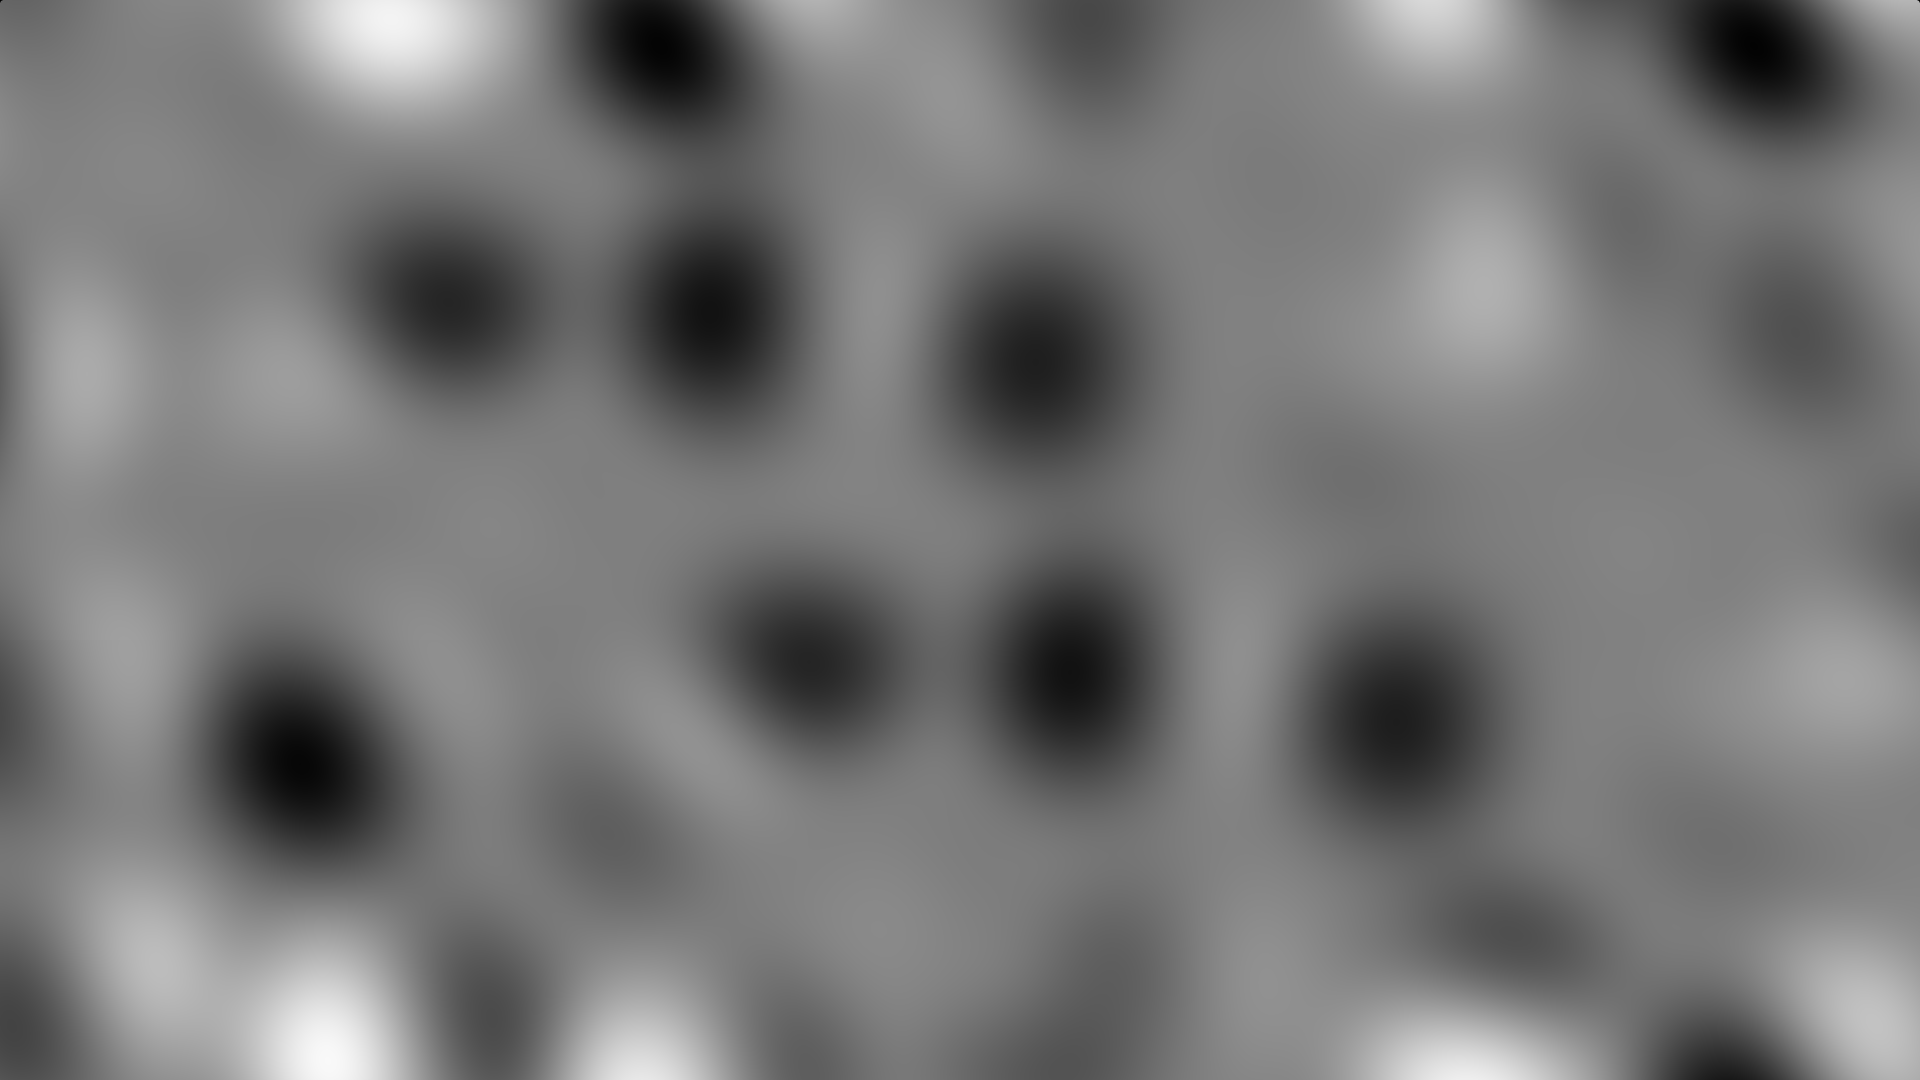
\includegraphics[width=.48\linewidth]{img/noise-simplex.png}%
        \fi
        \label{subfig:a}%
    }\hfill
    \subfloat[\centering Simplex noise \ac{fBm} from eq. \ref{eq:fbm1}, with coordinate offset $\vec{o} = \vec{0}$ and parameters $g = \frac{1}{l} = 1.5, k = 5$.]{%
        \ifgraphics
            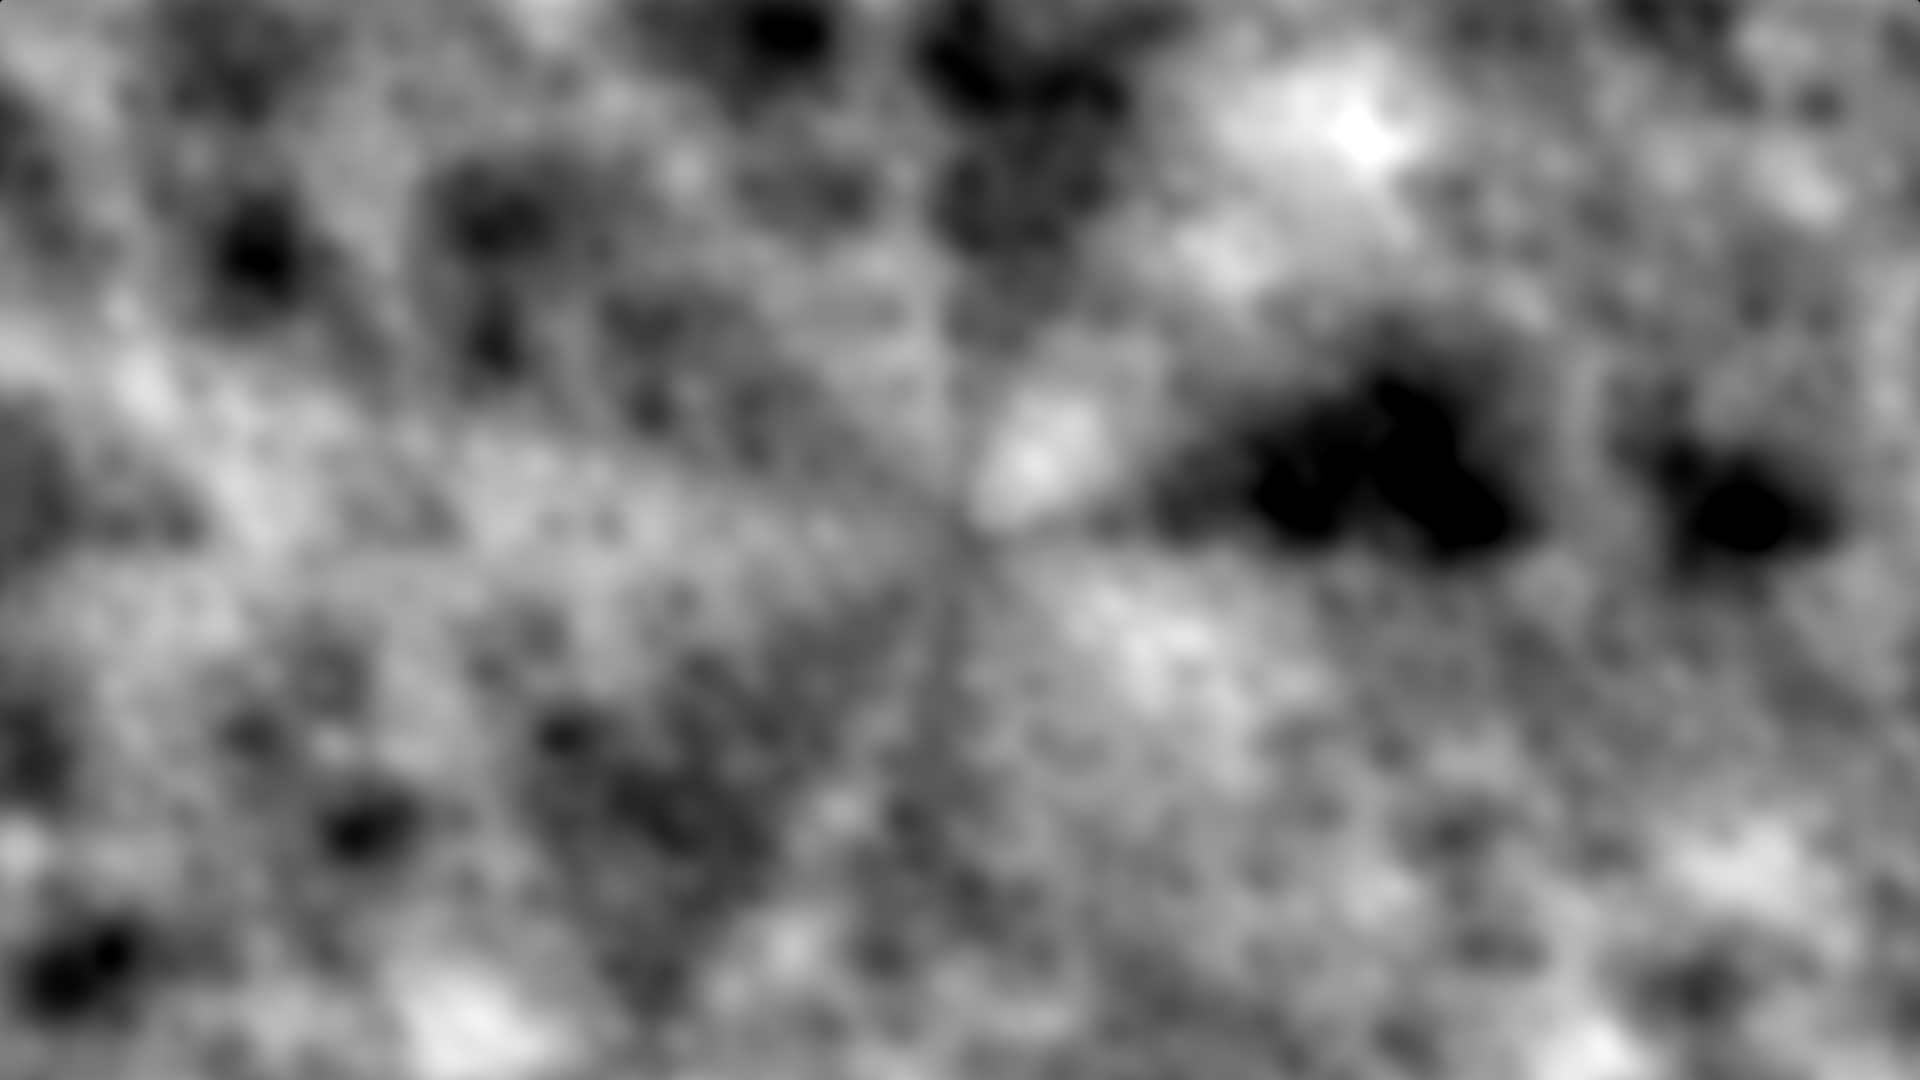
\includegraphics[width=.48\linewidth]{img/noise-fbm-coordinate-nooffset.png}%
        \fi
        \label{subfig:b}%
    }\\
    \subfloat[\centering Simplex noise \ac{fBm} from eq. \ref{eq:fbm1}, with non-zero coordinate offset $\vec{o} \ne \vec{0}$ and parameters $g = \frac{1}{l} = 1.5, k = 5$.]{%
        \ifgraphics
            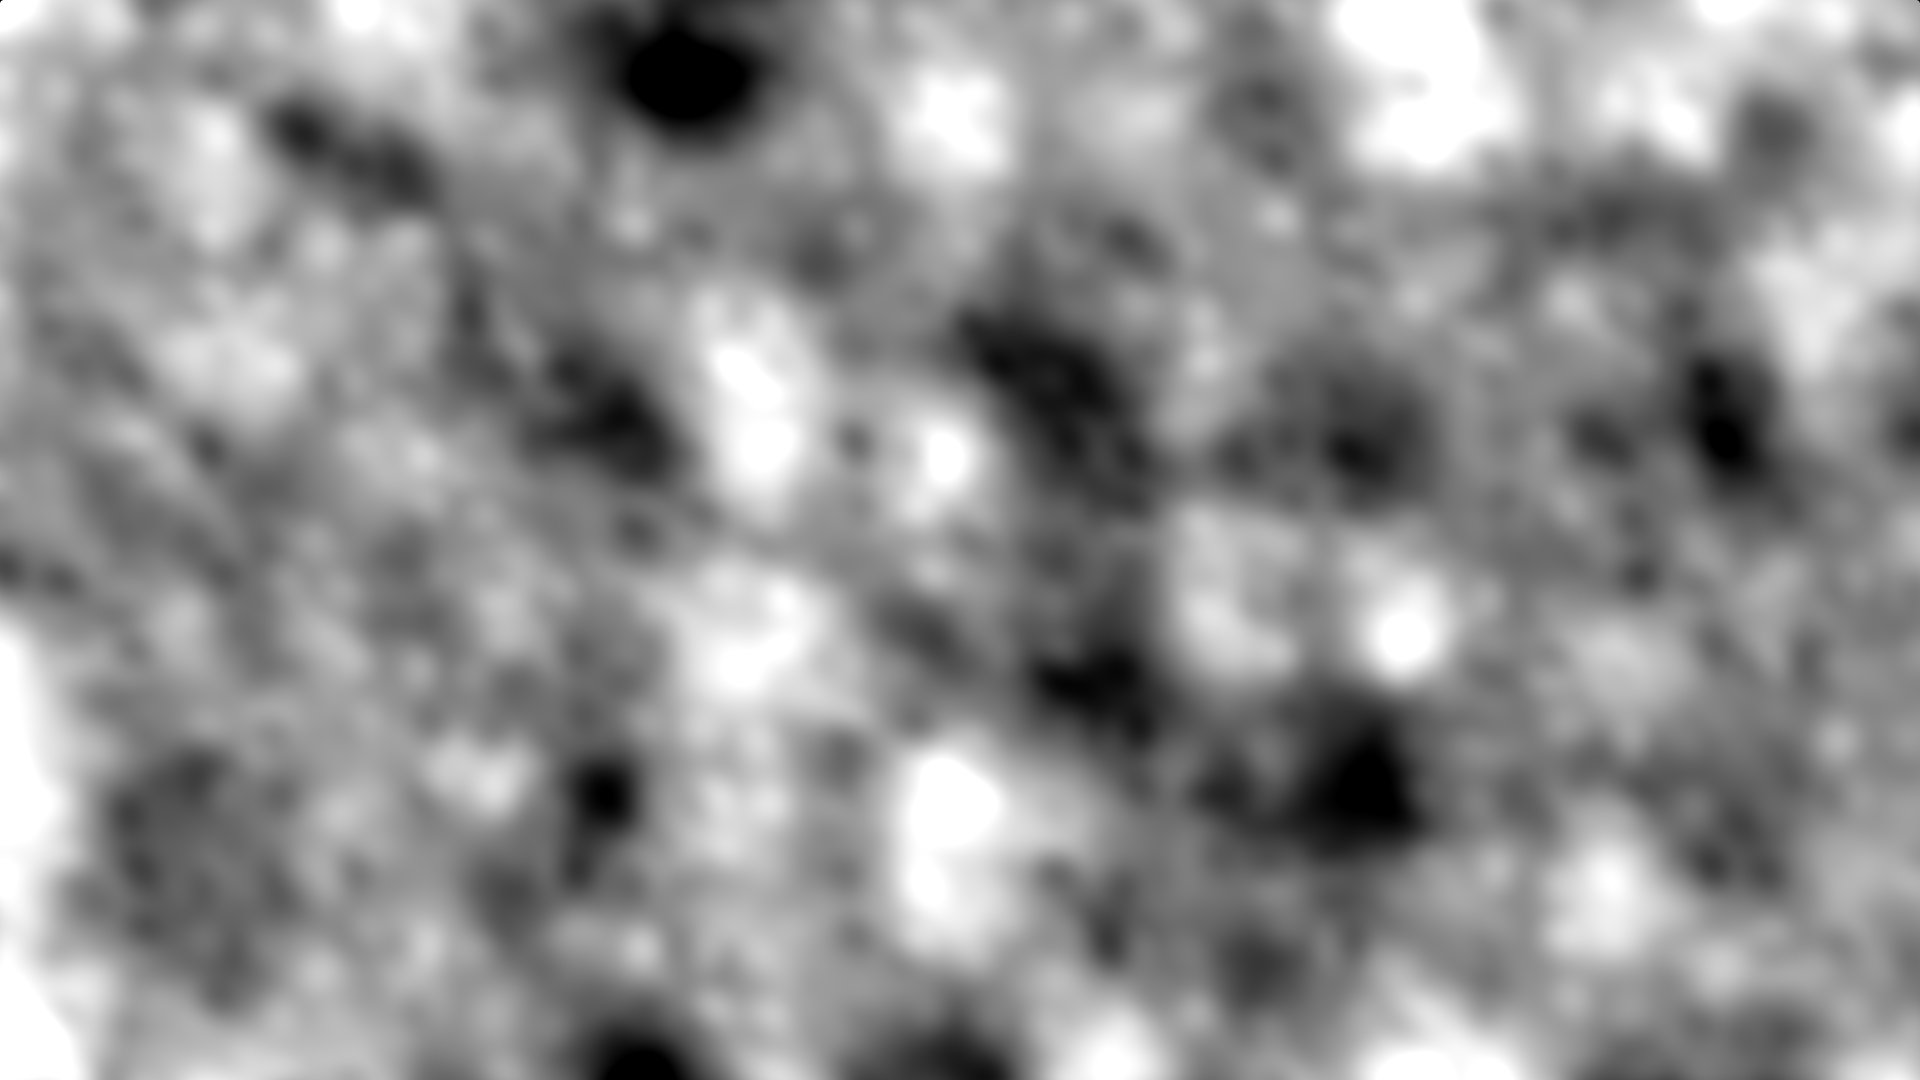
\includegraphics[width=.48\linewidth]{img/noise-fbm-coordinate-offset.png}%
        \fi
        \label{subfig:c}%
    }\hfill
    \subfloat[\centering Simplex noise \ac{fBm} with index offsets based on the distance to the center $r$, from eq. \ref{eq:fbm2}, with non-zero coordinate offset $\vec{o} \ne \vec{0}$ and parameters $a = g = \frac{1}{l} = 1.5, k = 5$.]{%
        \ifgraphics
            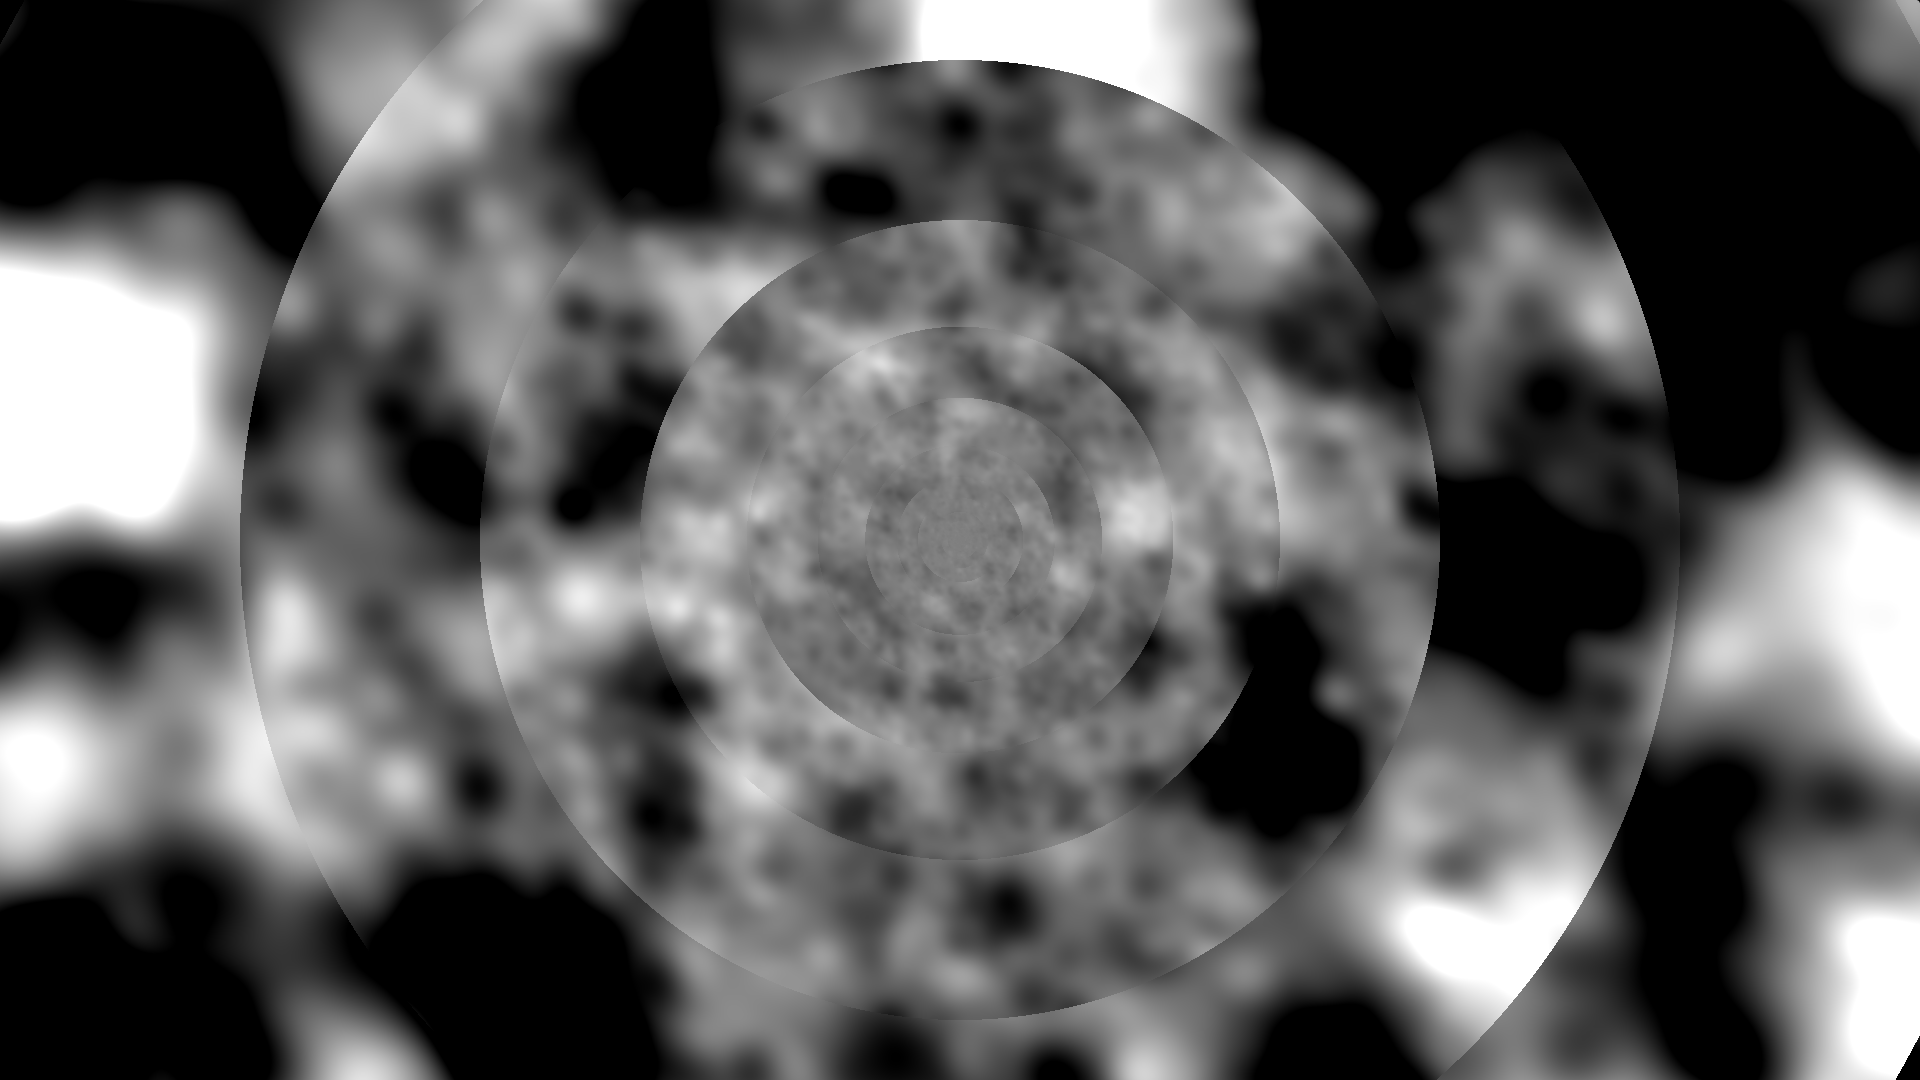
\includegraphics[width=.48\linewidth]{img/noise-octave-offset-integer.png}%
        \fi
        \label{subfig:d}%
    }
    \caption{Intermediate steps in the construction of the blended \ac{fBm} noise. Amplitude adjusted for visualization and clipped to range.}
    \label{fig:noise-demo-intermediate}
\end{figure}

Equation \ref{eq:fbm2} differs from equation \ref{eq:fbm1} in that we have added an index offset $j(r)$, which is computed from the distance to the \ac{HMD} $r$. Now we are able to offset the indices. However, this will result in noticeable discontinuities of the noise at the discontinuities of $j(r)$.

In order to remove these discontinuities, we shall introduce blending. Let us refer to the layers at indices $j(r), j(r) + 1, \dots, j(r) + k - 1$ as ``active layers'', the layer at index $j(r)$ as ``the first active layer'' and the layer at index $j(r) + k - 1$ as ``the last active layer''.

Let us define a weight function $w \colon \mathbb{Z} \times \mathbb{R} \to [0; 1]$, which will attenuate the first and last active layer, while leaving other layers unaffected.

\begin{equation}
    w(i, r) =
    \begin{cases}
        m(r) - j(r) = \{m(r)\} & \text{if } i = 0 \\
        1 - (m(r) - j(r)) = 1 - \{m(r)\} & \text{if } i = k \\
        1 & \text{otherwise}
    \end{cases}
\end{equation}

Where $\{ x \} = x - \lfloor x \rfloor$ is the upper fractional part of $x$.

\begin{equation}\label{eq:fbm3}
    \boxed{
        s' \coloneqq \frac{1}{k} \sum_{i=0}^{k} w(i, r) \cdot g^{i+j(r)} \cdot s\mleft(l^{i+j(r)} \begin{bmatrix}f_sx\\f_sy\\f_sz\\f_tt\end{bmatrix} + (i + j(r)) \vec{o}\mright)
    }
\end{equation}

Besides multiplying each layer by the weight $w(i, r)$, we have also changed the upper index of the sum from $k - 1$ to $k$, to account for the attenuation.

We have arrived at the derived general equation for blended \ac{fBm} noise based on distance $r$ with parameters $a, g, l \in \mathbb{R}; \vec{o} \in \mathbb{R}^n; k \in \mathbb{N}$. However, in general, this form does not satisfy our requirement of the amplitude being proportional to the distance $r$. In order for that to be true, we must set $a = g = \frac{1}{l}$.

\begin{figure}[ht]
    \centering
    \ifgraphics
        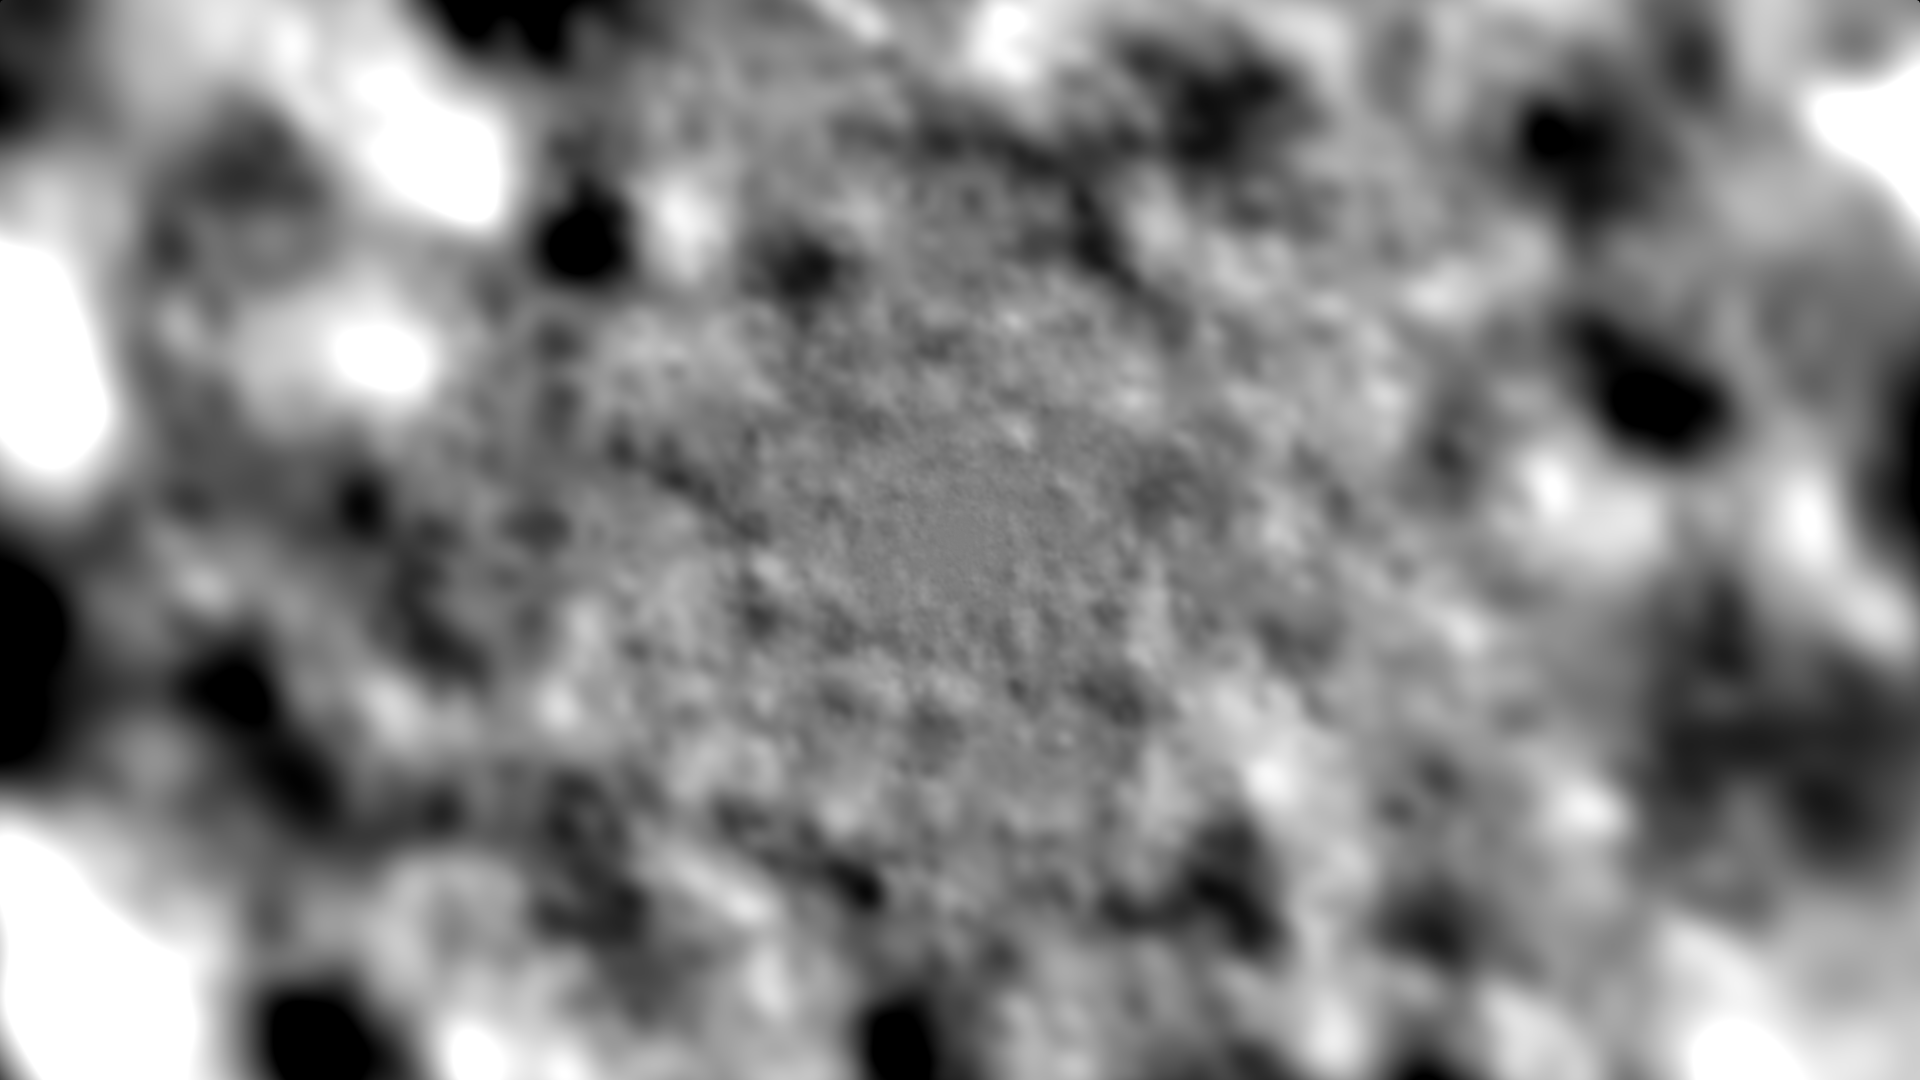
\includegraphics[width=\linewidth]{img/noise-final.png}%
    \fi
    \caption{The final implementation of the blended \ac{fBm} Simplex noise based on the distance to the center $r$, from eq. \ref{eq:fbm5}, with non-zero coordinate offset $\vec{o} \ne \vec{0}$ and parameters $a = g = \frac{1}{l} = 1.5, k = 5$. Amplitude adjusted for visualization.}
    \label{fig:noise-demo-final}
\end{figure}

The equation then expands to:

\begin{equation}\label{eq:fbm4}
    s' \coloneqq \frac{1}{k} \sum_{i=0}^{k} w(i, r) \cdot a^{i + \lfloor \log_a r \rfloor} \cdot s\mleft(a^{-(i + \lfloor \log_a r \rfloor)} \begin{bmatrix}f_sx\\f_sy\\f_sz\\f_tt\end{bmatrix} + (i + \lfloor \log_a r \rfloor) \vec{o}\mright)
\end{equation}
\begin{equation}
    w(i, r) =
    \begin{cases}
        \{\log_a r\} & \text{if } i = 0 \\
        1 - \{\log_a r\} & \text{if } i = k \\
        1 & \text{otherwise}
    \end{cases}
\end{equation}

Finally, we may or may not want the frequency of the fourth coordinate to be influenced by lacunarity. We reached better results when lacunarity did not affect the time coordinate.

\begin{equation}\label{eq:fbm5}
    \boxed{
        s' \coloneqq \frac{1}{k} \sum_{i=0}^{k} w(i, r) \cdot a^{i + \lfloor \log_a r \rfloor} \cdot s\mleft(\begin{bmatrix}a^{-(i + \lfloor \log_a r \rfloor)}f_sx\\a^{-(i + \lfloor \log_a r \rfloor)}f_sy\\a^{-(i + \lfloor \log_a r \rfloor)}f_sz\\f_tt\end{bmatrix} + (i + \lfloor \log_a r \rfloor) \vec{o}\mright)
    }
\end{equation}

This is the final equation used to sample blended \ac{fBm} noise based on the distance $r$ with parameters $a \in \mathbb{R}, \vec{o} \in \mathbb{R}^n, k \in \mathbb{N}$. This equation is used in the application to displace vertices of scene geometry. The result is scaled to ensure that no self-intersections of scene geometry occur.

\begin{figure}[H]
    \centering
    \ifgraphics
        {
            \def\constepsilon{0.001}
            \def\constymin{-10}
            \def\constymax{10}
            \def\constm{4}
            \def\consta{1.5}
            \def\fnf(#1){(ln(#1) / ln(\consta))}
            \def\fnfinv(#1){((\consta)^(#1))}
            \def\fnoctave(#1){(floor(\fnf(#1)))}
            \def\fnl(#1){(2 * \fnoctave(#1) - \fnf(#1) - \constm + 2)}

            \begin{tikzpicture}
                \begin{axis}[
                    xlabel={Distance from \ac{HMD}},
                    ylabel={Active Layer Indices},
                    samples=1000,
                    grid,
                    thick,
                    domain=0.0000001:30,
                    xmin=0,
                    xmax=30,
                    ymin=\constymin,
                    ymax=\constymax,
                    legend pos=outer north east,
                    no marks,
                    unit vector ratio={1, 1},
                    ytick = {-10, -5, 0, 5, 10},
                    minor y tick num=4,
                ]
                    \foreach \y in {\constymin, ..., \constymax}{
                        \def\boundleft{\fpeval{\fnfinv(\y + \constepsilon)}}
                        \def\boundright{\fpeval{\fnfinv(\y + 1 - \constepsilon)}}
                        \edef\temp{
                            \noexpand\fill[black!30!green, fill opacity=0.7] (\boundright, \y) -- plot[domain=\boundleft:\boundright, variable=\noexpand\x] ({\noexpand\x}, {\noexpand\fnf(\noexpand\x)}) -- (\boundright, \y);
                            \noexpand\fill[black!30!green, fill opacity=0.7] (\boundleft, {(\y) - (\constm - 1)}) -- plot[domain=\boundleft:\boundright, variable=\noexpand\x] ({\noexpand\x}, {\noexpand\fnl(\noexpand\x)}) -- (\boundleft, {(\y) - (\constm - 1)});
                        }
                        % \show\temp %-- uncomment this to see what the \temp macro does
                        \temp
                    }

                    \addplot+[draw=none, name path=fnf] {\fnf(x)};
                    \addplot+[draw=none, name path=fnl] {\fnl(x)};

                    \addplot+[draw=black, solid, jump mark mid] {\fnoctave(x) - 0};
                    \addplot+[draw=black, solid, jump mark mid] {\fnoctave(x) - 1};
                    \addplot+[draw=black, solid, jump mark mid] {\fnoctave(x) - 2};
                    \addplot+[draw=black, solid, jump mark mid] {\fnoctave(x) - 3};
                \end{axis}
            \end{tikzpicture}
        }
    \fi
    \caption{Computation of active layers based on the distance from the \ac{HMD}. Active layers as solid black lines. Green areas correspond to the weight of the first and last currently active layer.}\label{fig:noise-octaves}
\end{figure}

\begin{figure}[H]
    \centering
    \ifgraphics
        {
            \def\constepsilon{0.001}
            \def\constymin{-13}
            \def\constymax{7}
            \def\constm{4}
            \def\consta{1.5}
            \def\fnf(#1){(ln(#1) / ln(\consta))}
            \def\fnfinv(#1){((\consta)^(#1))}
            \def\fnoctave(#1){(floor(\fnf(#1)))}

            \begin{tikzpicture}
                \begin{axis}[
                    xlabel={Distance from \ac{HMD}},
                    ylabel={Active Layer Amplitudes},
                    samples=1000,
                    grid,
                    thick,
                    domain=0.0000001:30,
                    xmin=0,
                    xmax=30,
                    ymin=0,
                    ymax=30,
                    legend pos=outer north east,
                    no marks,
                    unit vector ratio={1, 1},
                    % ytick = {-10, -5, 0, 5},
                    % minor y tick num=4,
                ]
                \addplot+[black!30!green, fill opacity=0.7] {x};
                \addplot+[draw=black, solid, jump mark mid] {\fnfinv((\fnoctave(x) - 0))};
                \addplot+[draw=black, solid, jump mark mid] {\fnfinv((\fnoctave(x) - 1))};
                \addplot+[draw=black, solid, jump mark mid] {\fnfinv((\fnoctave(x) - 2))};
                \addplot+[draw=black, solid, jump mark mid] {\fnfinv((\fnoctave(x) - 3))};
                \end{axis}
            \end{tikzpicture}
        }
    \fi
    \caption{Amplitudes of active layers based on the distance from the \ac{HMD}, for the case where $a = g = 1.5$. Active layers as solid black lines. The green line shows the direct proportionality of the maximum active layer amplitude and the distance from the \ac{HMD}.}\label{fig:noise-amplitudes}
\end{figure}

\subsubsection{Visual Drifting}

In this section, we describe the implementation of our replication of visual drifting, sometimes described as the ``breathing'' or ``morphing'' of objects \autocites{diaz2010sacred}{kleinman1977comparison}.

As with depth perception distortion, there are two ways of implementing this replication, depending on the coordinate system and stage of rendering affected -- world-space and screen-space.

Ideally, the realism of the final implementation should not be broken by:

\begin{enumerate}
    \item the rotation of the \ac{HMD};
    \item the movement of the \ac{HMD} up to regular walking speed;
    \item the fast movement of objects in the scene.
\end{enumerate}

We chose to avoid a screen-space implementation, because satisfying any of those requirements seemed very difficult. Nevertheless, we are confident that our world-space solution satisfies at least the first two of the requirements.

We can use procedural noise to offset vertices into arbitrary directions in 3 dimensional space, but we need to be careful so that we do not cause geometry to self-intersect. Thankfully, we have already solved this problem in the previous section, and we can use that noise function.

Let us consider the general equation \ref{eq:fbm3} with $a = g = \frac{1}{l}$, and denote the right-hand side expression as a vector field $S \colon \mathbb{R}^n \to \mathbb{R}$, where $n = 4$:

\begin{equation}
    S\mleft(\begin{bmatrix}x\\y\\z\\t\end{bmatrix}\mright) = \frac{1}{k} \sum_{i=0}^{k} w(i, r) \cdot g^{i+j(r)} \cdot s\mleft(l^{i+j(r)} \begin{bmatrix}f_sx\\f_sy\\f_sz\\f_tt\end{bmatrix} + (i + j(r)) \vec{o}\mright)
\end{equation}

Then, we have two ways of using this noise function to generate an offset vector $\vec{v} \in \mathbb{R}^3$.

\textbf{Option one.}\\We compose the offset vector $\vec{v}$ from three samples of $S$ with coordinate offset vectors $\vec{o}_{0}, \vec{o}_{1}, \vec{o}_{2} \in \mathbb{R}^4$ to ensure different samples (different seeds would also work).

\begin{equation}
    \vec{v} \coloneqq \mleft[ S\mleft(\begin{bmatrix}x\\y\\z\\t\end{bmatrix} + \vec{o}_0\mright) \enspace S\mleft(\begin{bmatrix}x\\y\\z\\t\end{bmatrix} + \vec{o}_1\mright) \enspace S\mleft(\begin{bmatrix}x\\y\\z\\t\end{bmatrix} + \vec{o}_2\mright) \mright]^T
\end{equation}

\textbf{Option two.}\\We use the first 3 components of the gradient of $S$ as the offset vector $\vec{v}$.

\begin{equation}
    \vec{v} \coloneqq \begin{bmatrix}1&0&0&0\\0&1&0&0\\0&0&1&0\end{bmatrix} \nabla S\mleft(\begin{bmatrix}x\\y\\z\\t\end{bmatrix}\mright)
\end{equation}

\begin{figure}[htb]
    \centering
    \ifgraphics
        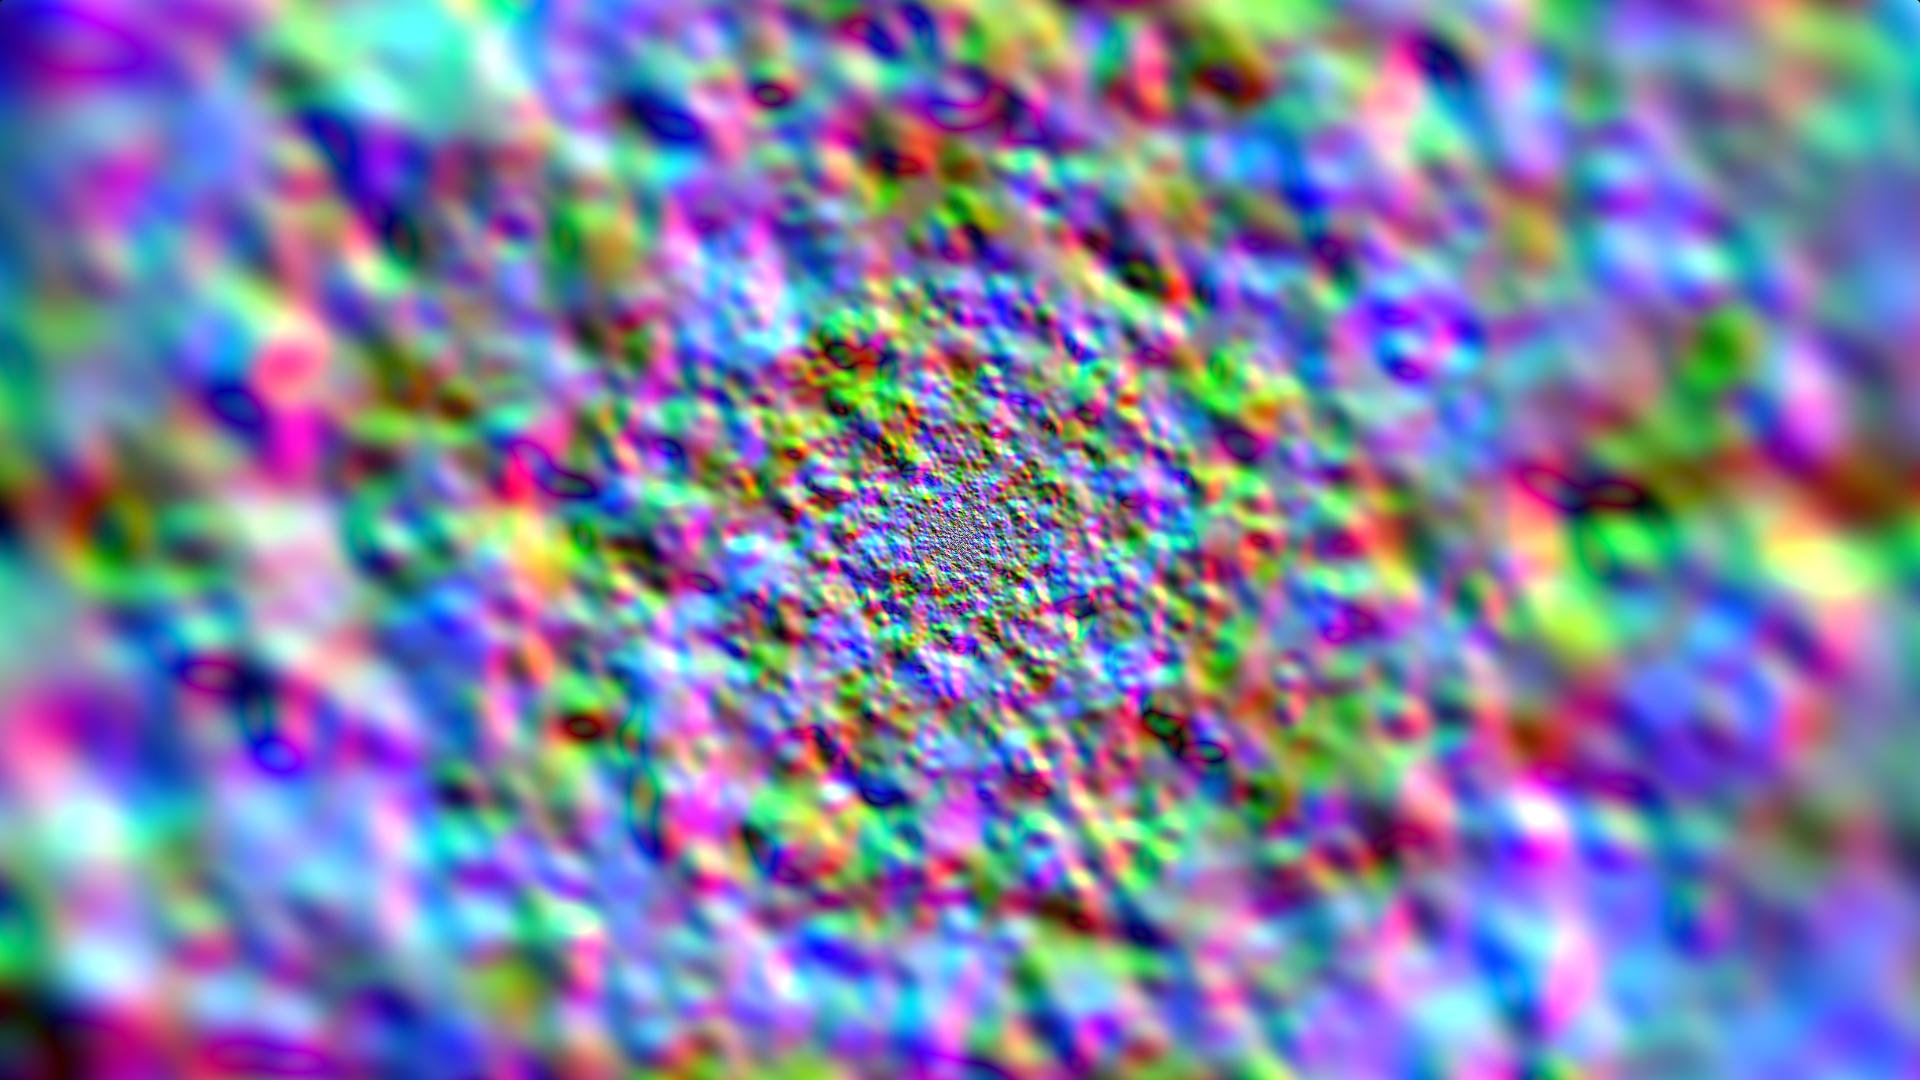
\includegraphics[width=\linewidth]{img/noise-grad-original.png}%
    \fi
    \caption{The first 3 components of the simplified gradient of the blended \ac{fBm} simplex noise $S_G$, from eq. \ref{eq:grad2}, with non-zero coordinate offset $\vec{o} \ne \vec{0}$ and parameters $a = g = \frac{1}{l} = 1.5, k = 5$. Components visualized as channels of the additive RGB color space. Amplitude adjusted for visualization and clipped to range.}
    \label{fig:noise-grad-original}
\end{figure}

The second option seems much more elegant, does not require 3 samples, and may even yield nicer results. Option two was our choice.

Unfortunately, the distance from the \ac{HMD} $r$ is dependent on the $x$, $y$ and $z$ coordinates, which makes the gradient overly complex. For that reason, we have decided to simplify the gradient by treating the $r$ parameter as a constant. We shall denote this simplification of the gradient $\nabla S$ as $S_G \colon \mathbb{R}^n \to \mathbb{R}^n$.

\begin{gather}
    S_G\mleft(\begin{bmatrix}x\\y\\z\\t\end{bmatrix}\mright) = \frac{1}{k} \sum_{i=0}^{k} w(i, r) g^{i+j(r)} \nabla s\mleft(l^{i+j(r)} \begin{bmatrix}f_sx\\f_sy\\f_sz\\f_tt\end{bmatrix} + (i + j(r)) \vec{o}\mright) \odot \begin{bmatrix}f_s\\f_s\\f_s\\f_t\end{bmatrix} l^{i+j(r)}\\
    = \begin{bmatrix}f_s\\f_s\\f_s\\f_t\end{bmatrix} \odot \mleft( \frac{1}{k} \sum_{i=0}^{k} w(i, r) g^{i+j(r)} \nabla s\mleft(l^{i+j(r)} \begin{bmatrix}f_sx\\f_sy\\f_sz\\f_tt\end{bmatrix} + (i + j(r)) \vec{o}\mright) l^{i+j(r)} \mright) \label{eq:grad1}
\end{gather}

The $\odot$ operator is the component-wise vector multiplication. For $g = \frac{1}{l}$, we could simplify further:

\begin{equation}\label{eq:grad2}
    S_G\mleft(\begin{bmatrix}x\\y\\z\\t\end{bmatrix}\mright) = \begin{bmatrix}f_s\\f_s\\f_s\\f_t\end{bmatrix} \odot \mleft( \frac{1}{k} \sum_{i=0}^{k} w(i, r) \nabla s\mleft(l^{i+j(r)} \begin{bmatrix}f_sx\\f_sy\\f_sz\\f_tt\end{bmatrix} + (i + j(r)) \vec{o}\mright) \mright)
\end{equation}

\begin{figure}[htb]
    \centering
    \ifgraphics
        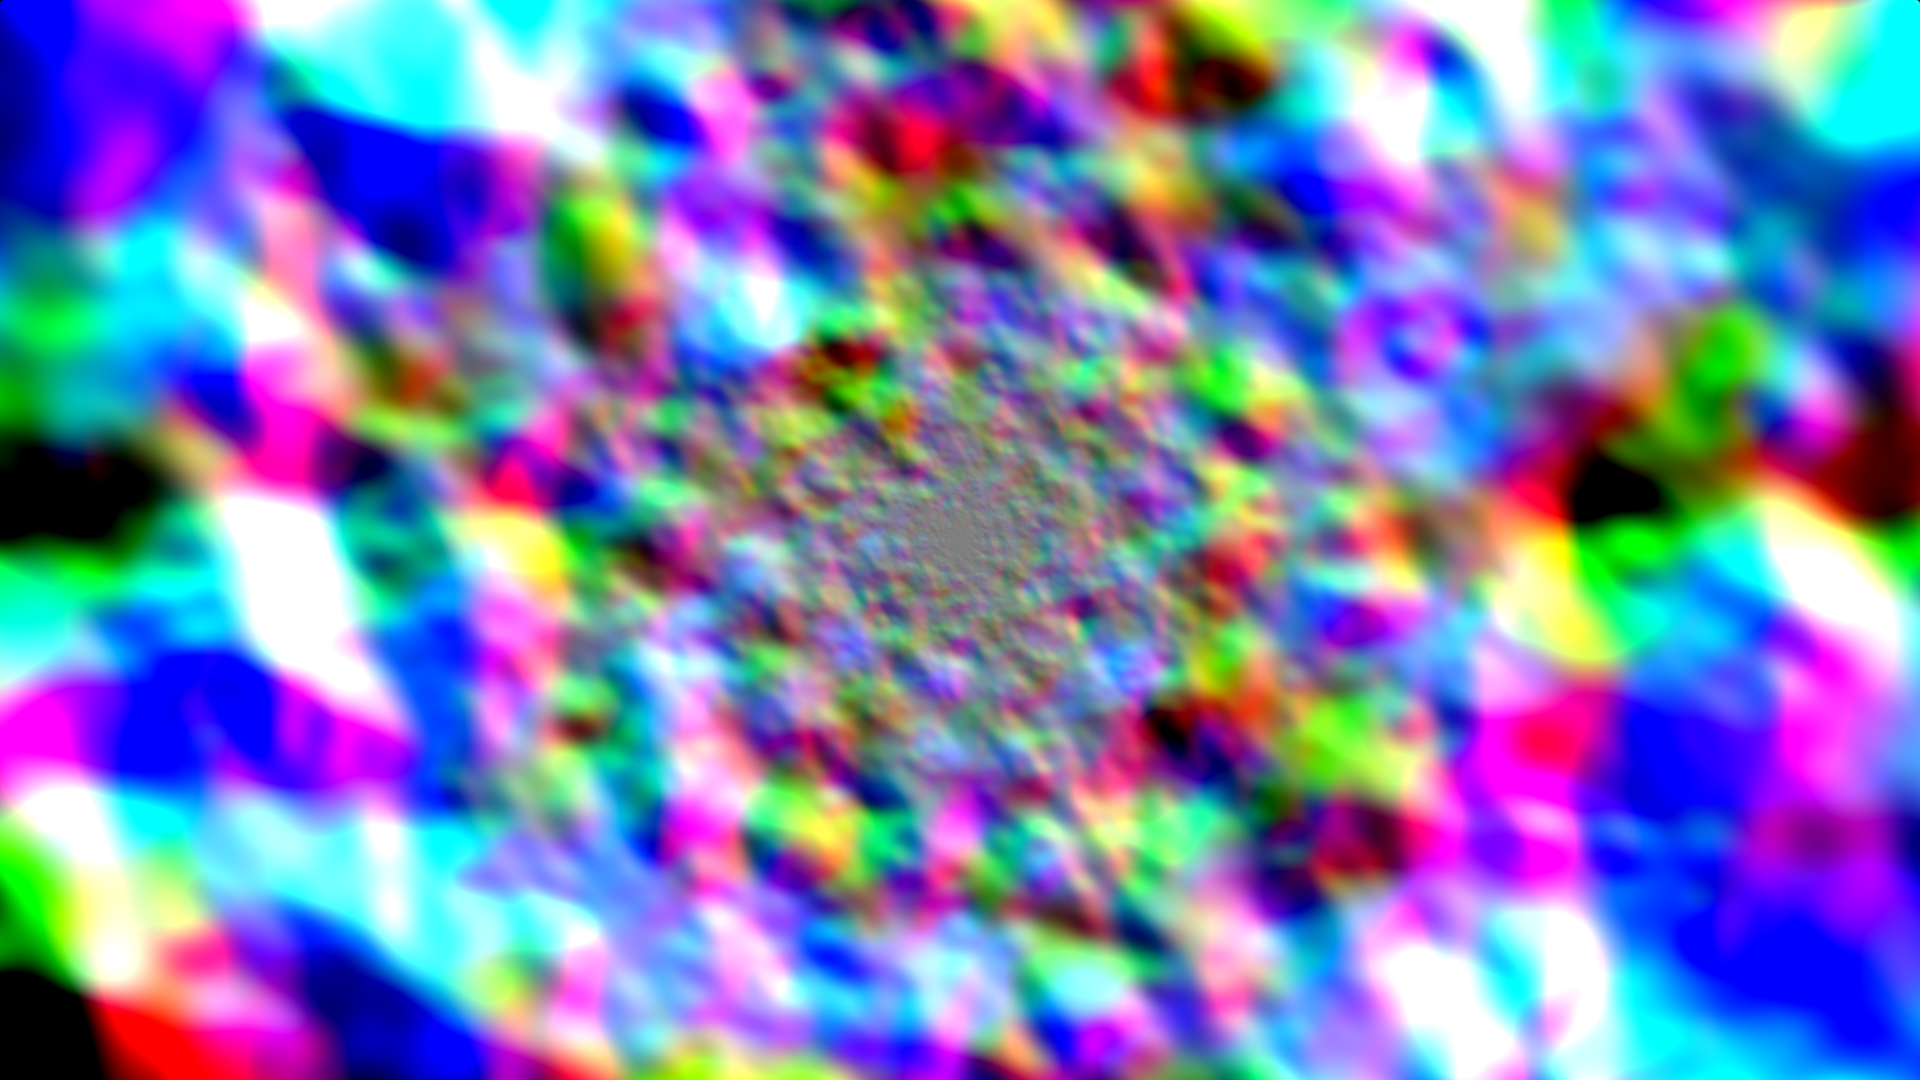
\includegraphics[width=\linewidth]{img/noise-grad-modulated.png}%
    \fi
    \caption{The first 3 components of the simplified gradient of the blended \ac{fBm} simplex noise $S'_G$, from eq. \ref{eq:grad3}, with non-zero coordinate offset $\vec{o} \ne \vec{0}$ and parameters $a = g = \frac{1}{l} = 1.5, k = 5$. Components visualized as channels of the additive RGB color space. Amplitude adjusted for visualization and clipped to range.}
    \label{fig:noise-grad-modulated}
\end{figure}

As we can see in figure \ref{fig:noise-grad-original}, the direct proportionality of the amplitude and the distance $r$ has been lost. We could have also noticed the $g^{i+j(r)}$ term being cancelled during the simplification step to equation \ref{eq:grad2}. In order to recover it, we need to divide the right-hand side of equation \ref{eq:grad1} by $l^{i+j(r)}$.

\begin{equation}\label{eq:grad3}
    S'_G\mleft(\begin{bmatrix}x\\y\\z\\t\end{bmatrix}\mright) = \begin{bmatrix}f_s\\f_s\\f_s\\f_t\end{bmatrix} \odot \mleft( \frac{1}{k} \sum_{i=0}^{k} w(i, r) g^{i+j(r)} \nabla s\mleft(l^{i+j(r)} \begin{bmatrix}f_sx\\f_sy\\f_sz\\f_tt\end{bmatrix} + (i + j(r)) \vec{o}\mright) \mright)
\end{equation}

We denote this modulated version of the simplified gradient as $S'_G$. As seen in figure \ref{fig:noise-grad-modulated}, the proportionality is recovered.

This is the final function we have used in our application to displace vertices of the scene geometry. To recapitulate the requirements we have placed upon ourselves to implement this replication, we required the realism not to be broken by the following actions.

\begin{enumerate}
    \item[$\boxtimes$] The rotation of the \ac{HMD}. Does not influence the sampling in any way, only the location of the \ac{HMD} is relevant. Success.
    \item[$\boxtimes$] The movement of the \ac{HMD} up to regular walking speed. The movement of the \ac{HMD} makes objects shift their active layers in a continuous, smooth way. Success.
    \item[$\square$] The fast movement of objects in the scene. Objects moving fast across the screen(s) might appear to morph erratically, significantly faster than the animation speed of still objects. Not ideal.
\end{enumerate}

Regarding the last point, one might think to modulate the vertex offset by the object's inverse velocity to account for the erratic animation, however, that might result in the object intersecting with the rest of the scene -- for example, with a static wall unaffected by the modulation.

We did not expect any fast-moving objects in the scene, and so this implementation was sufficient for our application.

\subsection{Non-Spatial Effects}
\subsubsection{Visual Acuity Enhancement}

\autocites{kluver1942mechanisms}{kluver1966mescal}{dittrich1998standardized}{diaz2010sacred}{siegel1975drug}{fischer1969effects}

\begin{figure}[H]
    \centering
    \ifgraphics
        \begin{tikzpicture}[node distance = 2cm, auto]
            \tikzstyle{block} = [rectangle, draw, fill=blue!20, text centered, rounded corners, minimum height=1em]
            \tikzstyle{line} = [draw, -latex']

            \node [block] (verticalblur) {Vertical Gaussian Blur};
            \node [block, below=1.25cm of verticalblur] (horizontalblur) {Horizontal Gaussian Blur};
            \node [block, below=0.5cm of horizontalblur] (unsharpmasking) {Unsharp Masking};

            \node [draw, densely dotted, minimum width=12cm, inner sep=0.5cm, fit=(verticalblur)] (pass1) {};
            \node [draw, densely dotted, minimum width=12cm, inner sep=0.5cm, fit=(horizontalblur)(unsharpmasking)] (pass2) {};

            \node [below right, text width=0.5\textwidth] at (pass1.north west) {{\scriptsize Render Pass A}};
            \node [below right, text width=0.5\textwidth] at (pass2.north west) {{\scriptsize Render Pass B}};

            \path [line] (verticalblur) -> (horizontalblur);
            \path [line] (horizontalblur) -> (unsharpmasking);
        \end{tikzpicture}
    \fi
    \caption{Execution order of distinct components of the sharpening effect.}\label{fig:sharpening}
\end{figure}

\subsubsection{Tracers}

\autocites{hartman1963effect}{diaz2010sacred}{anderson1972trifluoperazine}{kleinman1977comparison}

\begin{figure}[H]
    \centering
    \ifgraphics
        \tikzset{%
          block/.style  = {draw, thick, rectangle, minimum height = 3em, minimum width = 3em},
          op/.style     = {draw, circle, inner sep=-5mm},
          input/.style  = {draw, circle, minimum size=2mm, inner sep=0},
          output/.style = {input},
        }

        \begin{tikzpicture}[auto, thick, >=triangle 45]
            \draw node at (2, 6) [coordinate] (n13) {};
            \draw node at (4, 2) [coordinate] (n21) {};
            \draw node at (0, 6) [input, label={\small Input Frame}] (input) {};
            \draw node at (8, 4) [output, label={\small Modified Frame}] (output) {};
            \draw node at (2, 4) [op, label={left:$1 - \beta^{\Delta t}$}] (n12) {\Large $\times$};
            \draw node at (2, 2) [op] (n11) {\Large $+$};
            \draw node at (2, 0) [op, label={left:$\beta^{\Delta t}$}] (n10) {\Large $\times$};
            \draw node at (6, 6) [op, label={right:$1 - \alpha$}] (n33) {\Large $\times$};
            \draw node at (6, 4) [op] (n32) {\Large $+$};
            \draw node at (6, 2) [op, label={right:$\alpha$}] (n31) {\Large $\times$};
            \draw node at (4, 0) [block, label={right:\small Accumulation Texture}] (accumulator) {\Large $A$};

            \draw[->] (input) -- (n33);
            \draw[->] (n13) -- (n12);
            \draw[->] (n12) -- (n11);
            \draw[->] (n10) -- (n11);
            \draw[->] (accumulator) -- (n10);
            \draw[->] (n33) -- (n32);
            \draw[->] (n31) -- (n32);
            \draw[->] (n11) -- (n31);
            \draw[->] (n21) -- (accumulator);
            \draw[->] (n32) -- (output);
        \end{tikzpicture}
    \fi
    \caption{Execution graph of the tracer effect. The parameter $\alpha \in [0; 1]$ is the total opacity of the effect. The parameter $\beta \in [0; 1]$ is the feedback modifier corresponding to the ``duration'' of the resulting blur. Finally, $\Delta t$ is the time since the previous frame, making the effect less influenced by framerate fluctuations.}\label{fig:tracers-graph}
\end{figure}

\begin{figure}[H]
    \centering
    \ifgraphics
        \begin{tikzpicture}[node distance = 2cm, auto]
            \tikzstyle{block} = [rectangle, draw, fill=blue!20, text centered, rounded corners, minimum height=1em]
            \tikzstyle{line} = [draw, -latex']

            \node [block, dashed, draw=gray, fill=none] (unsharpmasking) {Unsharp Masking};
            \node [block, below=0.5cm of unsharpmasking] (tracers) {Tracers};

            \node [draw, densely dotted, minimum width=12cm, inner sep=0.5cm, fit=(unsharpmasking)(tracers)] (pass2) {};

            \node [below right, text width=0.5\textwidth] at (pass2.north west) {{\scriptsize Render Pass B (Continued)}};

            \path [line] (unsharpmasking) -> (tracers);
        \end{tikzpicture}
    \fi
    \caption{The tracer effect is applied in the second render pass of the sharpening effect.}\label{fig:tracers-order}
\end{figure}

\section{Complex Replication}
\subsection{Execution Order}

\begin{figure}[H]
    \centering
    \ifgraphics
        \begin{tikzpicture}[node distance = 2cm, auto]
            \tikzstyle{block} = [rectangle, draw, fill=blue!20, text centered, rounded corners, minimum height=1em]
            \tikzstyle{line} = [draw, -latex']

            \node [block] (wiggle) {Object Waviness};
            \node [block, below=0.5cm of wiggle] (depthperception) {Depth Perception Distortion};
            \node [block, below=1.25cm of depthperception] (sharpen) {Sharpening};
            \node [block, below=0.5cm of sharpen] (tracers) {Tracers};
            \node [block, below=1.25cm of tracers] (contrast) {Contrast and Saturation};

            \node [draw, densely dotted, minimum width=12cm, inner sep=0.5cm, fit=(wiggle)(depthperception)] (scopematerial) {};
            \node [draw, densely dotted, minimum width=12cm, inner sep=0.5cm, fit=(sharpen)(tracers)] (scopeplugin) {};
            \node [draw, densely dotted, minimum width=12cm, inner sep=0.5cm, fit=(contrast)] (scopeengine) {};

            \node [below right, text width=0.5\textwidth] at (scopematerial.north west) {{\scriptsize Material Graph\\Vertex Shader}};
            \node [below right, text width=0.5\textwidth] at (scopeplugin.north west) {{\scriptsize Engine Plugin Modifying the \acs{RDG}\\Post-Processing}};
            \node [below right, text width=0.5\textwidth] at (scopeengine.north west) {{\scriptsize Engine Built-in\\Post-Processing}};

            \path [line] (wiggle) -> (depthperception);
            \path [line] (depthperception) -> (sharpen);
            \path [line] (sharpen) -> (tracers);
            \path [line] (tracers) -> (contrast);
        \end{tikzpicture}
    \fi
    \caption{The execution order of partial replications, making up the complex replication.}\label{fig:scene-preview}
\end{figure}

\subsection{Experiment Automation}\label{sec:experiment_automation}
